% Originally: content/week-02.tex, \section{Metric spaces} (Corsin Week 2, Monday)

\section{Metric spaces}
\label{sec:metric_spaces}

\begin{definition}[Metric space]
\label{def:metric_space}
A \newterm{metric space} (\germanterm{metrischer Raum}) $(X,d)$ is any set $X$ with a
\newterm{metric} (\germanterm{Metrik}) $d : X \times X \to \mathbb{R}_{\geq 0}$ such that for all
$x, y, z \in X$:
\begin{enumerate}[label=\textbf{(\alph*)}]
  \item \textbf{Definiteness:} $d(x,y) \geq 0$, with equality if and only if $x = y$. In words: the
    distance is non-negative, and a point has zero distance to itself.
  \item \textbf{Symmetry:} $d(x,y) = d(y,x)$, i.e., $x$ has the same distance to $y$ as $y$ to $x$.
  \item \textbf{Triangle inequality ($\Delta$-inequality):} $d(x,z) \leq d(x,y) + d(y,z)$ ---
    \qt{detours make the way longer}.
\end{enumerate}
\end{definition}

\begin{ainote}
Corsin's gloss on definiteness reads \qt{the distance positive}; the formula $d \geq 0$ is
correct, but the gloss omits the ``non-''. Corrected in the prose above.
\end{ainote}

\begin{center}
\begin{tikzpicture}[>=Latex]
\draw[->] (-0.3,0) -- (4.2,0);
\draw[->] (0,-0.3) -- (0,3);
\coordinate (x) at (0.2,0.2);
\coordinate (y) at (1.6,2.0);
\coordinate (z) at (3.6,2.3);
\draw[blue,thick,->] (x) -- (y);
\draw[blue,thick,->] (y) -- (z);
\draw[red,thick,->] (x) -- (z);
\fill (x) circle (1.5pt) node[below]{$x$};
\fill (y) circle (1.5pt) node[above]{$y$};
\fill (z) circle (1.5pt) node[above]{$z$};
\node[red] at (2.3,0.7) {\footnotesize $d(x,z)$};
\node[blue] at (0.6,1.3) {\footnotesize $d(x,y)$};
\node[blue] at (2.7,2.4) {\footnotesize $d(y,z)$};
\node[red,below] at (2,-0.6) {\small $d(x,z) \le d(x,y)+d(y,z)$};
\end{tikzpicture}
\end{center}

% Generator: Claude Opus 5 (Medium)
\begin{aiexample}[Each axiom rules out something, and none is redundant]
\label{ex:metric_axioms_are_needed}
Three functions on $\mathbb{R}$, each failing exactly one axiom of
\Cref{def:metric_space}. It is worth checking these once: a definition only becomes memorable
once you know what it is keeping out.
\begin{enumerate}[label=\textbf{(\alph*)}]
  \item \textbf{Definiteness fails:} $d(x,y) := |x^2-y^2|$. This is symmetric and satisfies the
    triangle inequality (it is $|\cdot|$ composed with $x \mapsto x^2$), but
    $d(-1,1) = 0$ while $-1 \neq 1$. Distinct points at distance zero: the space cannot tell
    $-1$ from $1$, and no sequence could ever have a unique limit.
  \item \textbf{Symmetry fails:} $d(x,y) := \max\{\,y-x,\ 2(x-y)\,\}$, i.e.\ moving to the right
    costs $1$ per unit and moving to the left costs $2$. Here $d(0,1)=1$ but $d(1,0)=2$, so the
    return trip is more expensive than the outward one. Definiteness still holds ---
    $d(x,y) = 0$ forces $y-x \leq 0 \leq y-x$, hence $x=y$ --- and so does the triangle
    inequality, since $d(x,y) = \varphi(y-x)$ for $\varphi(t) := \max\{t,-2t\}$, and $\varphi$
    is a maximum of two linear functions vanishing at $0$, hence convex and positively
    homogeneous, hence subadditive. (Such a $d$ is called a \newterm{quasi-metric} and is
    genuinely useful elsewhere --- but $B_r(x)$ would then depend on which argument the centre
    sits in.)
  \item \textbf{Triangle inequality fails:} $d(x,y) := (x-y)^2$. Definiteness and symmetry are
    clear, but
    \[d(0,2) = 4 \quad > \quad d(0,1)+d(1,2) = 1+1 = 2,\]
    so the detour through $1$ is \emph{shorter} than going direct --- exactly the
    \qt{detours make the way longer} slogan reversed.
\end{enumerate}
\end{aiexample}

\subsection{Examples}

% Transition: Claude Opus 5 (High)
Three axioms are few enough that a great many things qualify as metrics, and the point of the
list below is exactly that breadth. Two of the examples are not what one would draw on a
blackboard as \qt{distance}: the discrete metric measures nothing but \qt{same or different},
and the supremum metric measures the distance between two \emph{functions}. Both are legitimate,
and it is worth letting them stretch the intuition now --- the second, in particular, is the
setting in which uniform convergence turns out to be an ordinary case of
\cref{def:convergent_sequence} (\cref{ex:uniform_convergence}).

% Source: Corsin Nick/Class Notes/Week 2.pdf, pp. 1--13
\begin{example}[Standard metrics on $\mathbb{R}^n$]
\label{ex:metric_examples}
\begin{enumerate}[label=\textbf{(\alph*)}]
  \item Let $X$ be a set. The \newterm{discrete metric} is given by
    \[d(x,y) := \begin{cases} 1 & \text{if } x \neq y \\ 0 & \text{if } x = y \end{cases}\]
    Important for counterexamples!
  \item Let $X := \mathbb{R}^n$. Then we have many choices for a metric; some common ones are:
  \begin{enumerate}[label=\textbf{(\roman*)}]
    \item \textbf{Manhattan metric:}
      \[d_1(x,y) := |x_1 - y_1| + \dots + |x_n - y_n| = \sum_{k=1}^{n} |x_k - y_k|\]
    \item \textbf{Standard metric:}
      \[d_2(x,y) := \sqrt{(x_1-y_1)^2 + \dots + (x_n-y_n)^2} = \sqrt{\sum_{k=1}^{n}(x_k - y_k)^2}\]
    \item \textbf{Supremum metric:}
      \[d_3(x,y) := \sup_{k = 1,\dots,n} |x_k - y_k|\]
  \end{enumerate}
\end{enumerate}
\end{example}

\begin{center}
\begin{tikzpicture}[>=Latex, scale=1.1]
  \draw[->] (-0.3,0) -- (4.5,0) node[right] {$x_1$};
  \draw[->] (0,-0.3) -- (0,3.5) node[above] {$x_2$};
  \coordinate (X) at (0.8, 0.8);
  \coordinate (Y) at (3.8, 2.8);
  \coordinate (Corner) at (3.8, 0.8);

  \draw[dotted, gray] (0, 0.8) node[left, font=\footnotesize] {$x_2$} -- (X) -- (0.8, 0) node[below, font=\footnotesize] {$x_1$};
  \draw[dotted, gray] (0, 2.8) node[left, font=\footnotesize] {$y_2$} -- (Y) -- (3.8, 0) node[below, font=\footnotesize] {$y_1$};

  % The two legs are just coordinate differences -- neither one IS a metric.
  \draw[orange!90!black, ultra thick] (X) -- (Corner) -- (Y);
  \node[below, font=\small, orange!90!black] at (2.3,0.72) {$a := |x_1-y_1|$};
  \node[right, font=\small, orange!90!black] at (3.9,1.8) {$b := |x_2-y_2|$};

  \draw[blue!80!black, very thick] (X) -- (Y);
  \node[above left, font=\small, blue!80!black] at (2.9,2.1) {$d_2 = \sqrt{a^2+b^2}$};

  \fill (X) circle (2pt) node[above left] {$x$};
  \fill (Y) circle (2pt) node[above right] {$y$};

  % d_3 picks out the longer leg; here a > b.
  \draw[red!80!black, thick, <->] (0.8,-0.95) -- node[below, font=\small] {$d_3 = \max\{a,b\} = a$} (3.8,-0.95);
  \draw[red!80!black, dotted] (0.8,0) -- (0.8,-0.95);
  \draw[red!80!black, dotted] (3.8,0) -- (3.8,-0.95);

  \node[orange!90!black, font=\small, anchor=west] at (0.1,3.25) {$d_1 = a+b$ \ (the full orange path)};
\end{tikzpicture}
\end{center}

Note that $d_1$ is the \textbf{sum} of the two legs and $d_3$ the \textbf{larger} of them ---
neither is a single leg on its own. Only $d_2$ is the straight-line distance you would draw by
reflex.

In general,
\[
d(x,y) := \sqrt[m]{\sum_{k=1}^{n} (x_k - y_k)^m}
\]
is a metric on $\mathbb{R}^n$ for any $m$.

\begin{ainote}
Two caveats Corsin leaves out. The powers must be taken of \textbf{absolute values},
$\sqrt[m]{\sum_k|x_k-y_k|^m}$ --- otherwise for odd $m$ the radicand can be negative. And it is
a metric only for $m \geq 1$: for $m \in (0,1)$ the triangle inequality fails, as
\Cref{ex:4.3}\textbf{.6} shows with $x=e_1$, $y=e_2$, where
$|x+y|_m = 2^{1/m} > 2 = |x|_m+|y|_m$. Written as stated above.
\end{ainote}

\begin{example}[continued]
\begin{enumerate}[label=\textbf{(\alph*)}, start=3]
  \item Let $X := C^0([0,1], \mathbb{R})$ be the set of continuous functions $[0,1] \to \mathbb{R}$.
    Then we can define the \newterm{supremum metric} for $f, g \in X$:
    \[
    d(f,g) := \sup_{x \in [0,1]} |f(x) - g(x)|
    \]
    This is well defined --- i.e.\ the supremum is a real number and not $+\infty$ --- because
    $|f-g|$ is continuous on the compact interval $[0,1]$ and therefore bounded, by the extreme
    value theorem from \emph{Analysis I} (revisited in this generality as
    \cref{lem:sequential_compactness_extreme_values} below). Compactness of the domain is doing
    real work here: on $C^0(\mathbb{R},\mathbb{R})$ the same formula would produce $\infty$ for
    $f(x) := x$, $g := 0$.
  \item Let $X := S^2 := \{(x_1,x_2,x_3) \in \mathbb{R}^3 : x_1^2 + x_2^2 + x_3^2 = 1\}$. $S^n$ is
    called the \newterm{$n$-dimensional sphere}, or \newterm{$n$-sphere}. The closest path between
    two points on the sphere is an \textbf{arc of a great circle} (a \textit{geodesic}). This
    defines a metric, similar to how straight lines define a metric on $\mathbb{R}^n$.
\end{enumerate}
\end{example}

\begin{center}
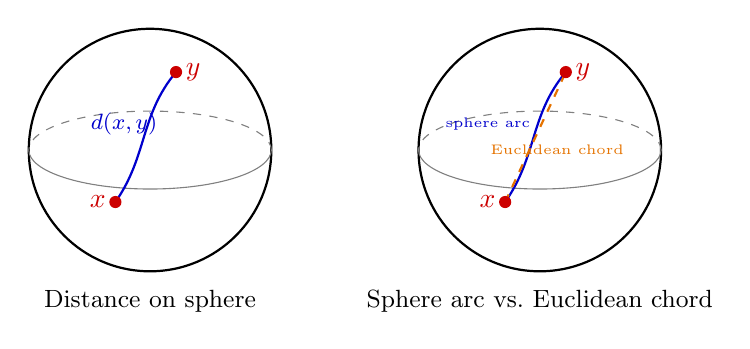
\begin{tikzpicture}[scale=1.1]
  \begin{scope}[shift={(0,0)}]
    \draw[thick] (0,0) circle (1.4);
    \draw[dashed, gray] (1.4,0) arc (0:180:1.4 and 0.45);
    \draw[gray] (-1.4,0) arc (180:360:1.4 and 0.45);
    \coordinate (x1) at (-0.4,-0.6);
    \coordinate (y1) at (0.3,0.9);
    \draw[blue!80!black, thick] (x1) to[out=55, in=230] (y1);
    \fill[red!80!black] (x1) circle (2pt) node[left] {$x$};
    \fill[red!80!black] (y1) circle (2pt) node[right] {$y$};
    \node[blue!80!black, font=\footnotesize] at (-0.3,0.3) {$d(x,y)$};
    \node[below, font=\small] at (0,-1.5) {Distance on sphere};
  \end{scope}

  \begin{scope}[shift={(4.5,0)}]
    \draw[thick] (0,0) circle (1.4);
    \draw[dashed, gray] (1.4,0) arc (0:180:1.4 and 0.45);
    \draw[gray] (-1.4,0) arc (180:360:1.4 and 0.45);
    \coordinate (x2) at (-0.4,-0.6);
    \coordinate (y2) at (0.3,0.9);
    \draw[blue!80!black, thick] (x2) to[out=55, in=230] (y2);
    \draw[orange!90!black, thick, dashed] (x2) -- (y2);
    \fill[red!80!black] (x2) circle (2pt) node[left] {$x$};
    \fill[red!80!black] (y2) circle (2pt) node[right] {$y$};
    \node[blue!80!black, font=\tiny] at (-0.6,0.3) {sphere arc};
    \node[orange!90!black, font=\tiny] at (0.2,0.0) {Euclidean chord};
    \node[below, font=\small] at (0,-1.5) {Sphere arc vs.\ Euclidean chord};
  \end{scope}
\end{tikzpicture}
\end{center}

\begin{exercise}[Supremum metric]
\label{ex:sup_metric_is_metric}
Show that the supremum metric from \cref{ex:metric_examples} \textbf{(c)} is a metric.
\end{exercise}

% Kept inline: solved directly in Corsin Nick/Class Notes/Week 2.pdf, p. 6.
\begin{exercisesolution}[Proof of \cref{ex:sup_metric_is_metric}]
Clearly, symmetry and definiteness hold. For the triangle inequality, let $f, g, h \in C^0([0,1])$ and
set $p := f - h$ and $q := h - g$. Then for all $x \in [0,1]$, we have:
\[|p(x)| \leq \sup|p| \qquad \text{and} \qquad |q(x)| \leq \sup|q|.\]
Adding the inequalities, we obtain for all $x \in [0,1]$:
\begin{align*}
|f(x) - g(x)| &= |p(x) + q(x)| \\
&\leq |p(x)| + |q(x)| \\
&\leq \sup|p| + \sup|q| \\
&= \sup|f - h| + \sup|h - g|.
\end{align*}
\end{exercisesolution}

% Quelle: Jérôme Paschoud/Notizen/Woche 2.1 Metrische Räume.pdf, p. 2
\begin{exercise}[$L^1$-metric]
\label{ex:integral_metric_is_metric}
Let $X := C^0([0,1], \mathbb{R})$ be the set of continuous functions $[0,1] \to \mathbb{R}$.
For $f,g \in X$, define
\[d(f,g) := \int_0^1 \lvert f(t)-g(t)\rvert\,dt.\]
Is $(X,d)$ a metric space? Provide a proof.
\end{exercise}

% Generator: Gemini 3.6 Pro
\begin{exercisesolution}[Proof of \cref{ex:integral_metric_is_metric}]
Yes, it is a metric space. We verify the three axioms of a metric:
\begin{enumerate}[label=\textbf{(\alph*)}]
  \item \textbf{Definiteness:} Clearly $d(f,g) \geq 0$ since the integrand $\lvert f(t)-g(t)\rvert$ is non-negative. If $f = g$, then $d(f,f) = \int_0^1 0\,dt = 0$. Conversely, suppose $d(f,g) = 0$. Since $\lvert f-g\rvert$ is a continuous, non-negative function, its integral over $[0,1]$ can only be zero if the integrand is identically zero. Thus $f(t) = g(t)$ for all $t \in [0,1]$, which means $f = g$.
  \item \textbf{Symmetry:} $d(f,g) = \int_0^1 \lvert f(t)-g(t)\rvert\,dt = \int_0^1 \lvert g(t)-f(t)\rvert\,dt = d(g,f)$.
  \item \textbf{Triangle inequality:} Let $f, g, h \in X$. The triangle inequality for real numbers yields $\lvert f(t)-h(t)\rvert \leq \lvert f(t)-g(t)\rvert + \lvert g(t)-h(t)\rvert$ for all $t \in [0,1]$. Integrating both sides, we obtain:
  \begin{align*}
  d(f,h) &= \int_0^1 \lvert f(t)-h(t)\rvert\,dt \\
  &\leq \int_0^1 \left(\lvert f(t)-g(t)\rvert + \lvert g(t)-h(t)\rvert\right)\,dt \\
  &= \int_0^1 \lvert f(t)-g(t)\rvert\,dt + \int_0^1 \lvert g(t)-h(t)\rvert\,dt \\
  &= d(f,g) + d(g,h).
  \end{align*}
\end{enumerate}
\end{exercisesolution}

% The old chapter closed here with a transition into "Open and closed sets"; that topic is now
% \cref{ch:open_closed}, whose own opening paragraph says the same thing, so the bridge is gone.

% --- exercises relocated here from the dissolved sheets ---

% Transition: Claude Opus 5 (Medium)
\begin{ainote}[Where the exercise-sheet problems live]
The official problem sheets are not reproduced as blocks anywhere in this document. Each problem
is quoted verbatim (from \texttt{exercises/ExN\_Analysis2\_eng.pdf}; attribution: Prof.\ Joaquim
Serra, D-MATH, ETH Z\"urich) and placed with the material it tests, so a problem from sheet 3 may
well appear several chapters away from a problem from sheet 2. Its solution is then in the
\emph{Solutions} section of that same chapter. Corsin's priority tags (\textbf{important},
\textbf{semi-important}, \textbf{optional}) and the official \textbf{(*)} difficulty marker are
carried along in each problem's title.
\end{ainote}

\begin{notation}
% Originally: content/exercise-sheets/week-02.tex, the sheet's own preamble.
Some problems in this document have a closed-answer format, similar to what you might find on the
final exam. \qt{Multiple Choice} means that zero, one or more answers can be correct. Questions
marked with (*) are a bit more complex, you might want to skip them at the first read.
\end{notation}

% Originally: content/week-02.tex, end of \section{Compactness}

\begin{aiexercise}[Equivalence of Manhattan and Supremum Metrics]
\label{ex:ai_metric_equivalence}
% Generator: Gemini 3.6 Flash (Medium)
Let $x := (x_1, x_2) \in \mathbb{R}^2$. Show that the Manhattan metric $d_1(x,0) := |x_1| + |x_2|$ and the supremum metric $d_3(x,0) := \max\{|x_1|, |x_2|\}$ satisfy the sharp inequalities:
\[
d_3(x,0) \leq d_1(x,0) \leq 2 \, d_3(x,0).
\]
\end{aiexercise}

% Originally: content/exercise-sheets/week-02.tex, problem 2.1
% Source: exercises/Ex2_Analysis2_eng.pdf, p. 1

\begin{exercise}[2.1 --- Examples and Non-examples of Metric spaces]
\label{ex:2.1}
Which of the following pairs are metric spaces? Prove it or provide a counterexample.
\begin{enumerate}[label=\textbf{\arabic*.}]
  \item $(B(X), d)$, where $B(X)$ denotes the set of all bounded functions from a non-empty set
    $X$ to $\mathbb{R}$ and
    $$d(f,g) := \sup_{x \in X} |f(x) - g(x)|.$$
  \item $(\mathbb{Q}_+, d)$, where $\mathbb{Q}_+$ are the positive rational numbers and
    $d(x,y) := \left|\tfrac{1}{x} - \tfrac{1}{y}\right|$.
  \item $(\mathbb{R}^2, d)$, where $d(x,y) := (x_1 - y_1)^2 + |x_2 - y_2|$.
  \item $(\mathbb{R}^2, d)$, where $d(x,y) := |x_1 - y_1|^{1/2} + |x_2 - y_2|$.
  \item $(\mathbb{R}^{n \times n}, d)$ with
    $d(X,Y) := \left(\Tr\{(X-Y)\transp(X-Y)\}\right)^{1/2}$.
  \item \textbf{(*)} $(\mathbb{R}^{n \times n}, d)$ with
    $$d(X,Y) := \sup\{|v\transp(X-Y)v| : v \in \mathbb{R}^n, \|v\| = 1\},$$
    and $\mathbb{R}^{n\times n}$ denoting the set of square matrices.
  \item \textbf{(*)} $(\mathbb{R}^2/\mathbb{Z}^2, d)$ where the flat 2-dimensional torus
    $\mathbb{R}^2/\mathbb{Z}^2$ is the set of equivalence classes of pairs of real numbers under
    the equivalence relation
    $$x, y \in \mathbb{R}^2, \quad x \sim y \iff x_1 - y_1 \in \mathbb{Z},\ x_2 - y_2 \in \mathbb{Z},$$
    and $d([x],[y]) := \inf_{k,h \in \mathbb{Z}} \|x - y + (k,h)\|$, with $\|\cdot\|$ denoting the
    Euclidean distance and $[x] \in \mathbb{R}^2/\mathbb{Z}^2$ denoting the equivalence class of
    $x \in \mathbb{R}^2$.
\end{enumerate}

\textit{Official hints:} \textbf{2.1.3} and \textbf{2.1.4} --- ignore what happens in the second
variable, it is there only to distract you. \textbf{2.1.5} --- rewrite, for a general matrix
$A := X - Y$, what $\Tr\{A\transp A\}^{1/2}$ actually means; it should look familiar.
\textbf{2.1.6} --- see what happens if $(X-Y)$ is anti-symmetric. \textbf{2.1.7} --- convince
yourself first that the ``inf'' is in fact a ``min''.
\end{exercise}

% Quelle: Diego Torres Tejeda/Notes - 02.03 - Diego Torres Tejeda.pdf, p. 2
\begin{ainote}[Diego's geometric intuition for the flat torus $\mathbb{R}^2/\mathbb{Z}^2$]
Diego's notes highlight the geometric picture behind part \textbf{2.1.7}: every equivalence class in $\mathbb{R}^2/\mathbb{Z}^2$ has a representative in $[0,1] \times [0,1]$. Identifying opposite boundaries $(0,x) \sim (1,x)$ and $(x,0) \sim (x,1)$ folds the unit square into a cylinder and subsequently into a 2D torus $\mathbb{T}^2 := \mathbb{R}^2/\mathbb{Z}^2$. The distance $d([x],[y])$ is simply the shortest Euclidean distance between points on this folded torus.
\end{ainote}

% Originally: content/exercise-sheets/week-02.tex, problem 2.5
% Source: exercises/Ex2_Analysis2_eng.pdf, p. 1

\begin{exercise}[2.5 --- Product of metric spaces]
\label{ex:2.5}
Let $(X, d_X)$ and $(Y, d_Y)$ be a pair of metric spaces. Recall that the set of ordered pairs
$(x,y)$ with $x \in X$ and $y \in Y$ is denoted by $X \times Y$. Consider the following functions
$X \times Y \to [0,\infty)$:
$$
\begin{aligned}
d_1((x,y),(x',y')) &:= \max\{d_X(x,x'), d_Y(y,y')\} \\
d_2((x,y),(x',y')) &:= d_X(x,x') + d_Y(y,y') \\
d_3((x,y),(x',y')) &:= \sqrt{d_X(x,x')^2 + d_Y(y,y')^2}.
\end{aligned}
$$
\begin{enumerate}[label=\textbf{\arabic*.}]
  \item Show that they are all valid distance functions on $X \times Y$.
  \item Show that they are all equivalent, i.e.\ there is a number $C > 0$ such that
    $$d_1((x,y),(x',y')) \leq C\,d_2((x,y),(x',y')) \leq C^2 d_3((x,y),(x',y')) \leq C^3 d_1((x,y),(x',y'))$$
    for all $x, x' \in X$, $y, y' \in Y$.
  \item Show that a sequence $(x_n, y_n) \to (x,y)$ with respect to $(X \times Y, d_3)$ if and
    only if $x_n \to x$ with respect to $d_X$ and $y_n \to y$ with respect to $d_Y$.
\end{enumerate}
\textit{Official hint:} don't get distracted by the abstract set-up --- you already know all
these things for $\mathbb{R} \times \mathbb{R}$; start from there, then rewrite those arguments in
this general framework.
\end{exercise}
